\section{Auswertung}
\label{sec:Auswertung}
Für die verschiedenen Messgeräte werden die folgenden Ungenauigkeiten angenommen.
\begin{align*}
	\sigma_R &= \SI{0.1}{\ohm}\\
	\sigma_U &= \SI{0.01}{\volt}\\
	\sigma_I &= \SI{0.1}{\milli\ampere}\\
	\sigma_{\symup\Delta t} &= \SI{0.1}{\second}	\,\text.
\end{align*}
Die Grafiken sowie Rechnungen werden mit Python erstellt bzw. durchgeführt \cite{python}.
\subsection{Bestimmung der verschiedenen Molwärme}
Die Molwärme bei konstantem $C_\mathrm{p}$ wird aus der zugeführten elektrischen Energie bestimmt.
Diese kann aus den Werten in Tabelle \ref{tab:tab1} mit
\begin{align}
	E &= U \cdot I \cdot \symup{\Delta} t,\\
	C_\mathrm{p} &= \frac{M}{m}\cdot\frac{E}{\symup{\Delta} T}
	\label{eqn:cp}
\end{align}
berechnet werden.
Dabei ist $E$ die zugeführte Energie, $U$ die Spannung, $I$ die Stromstärke, $\symup\Delta t$ die Dauer zwischen den Messpunkten, $\symup\Delta T$ der Temperaturunterschied zwischen den Messpunkten, $M$ die molare Masse von Kupfer und $m$ die Probenmasse. Die materialspezifischen Konstanten werden den Quellen \cite{Anleitung4} für die Molmasse von Kupfer, \cite{Anleitung5} für Kompressionsmodul und Dichte und zuletzt \cite[4]{Anleitung} für die Probenmasse, entnommen. Diese lauten:
\begin{align*}
  M &= \SI{0.0635}{\kilo\gram\mol^{-1}} \\
  \kappa &= \SI{140}{GPa} \\
  m &= \SI{0.342}{\kilo\gram} \\
  \rho &= \SI{8920}{\kilo\gram\meter^{-3}}
\end{align*}
In Tabelle \ref{tab:tab1} finden sich zu diesen Größen zusätzlich die berechneten Molwärmen.
\begin{table}
  \centering
  \caption{Daten für die Bestimmung der Molwärme bei konstantem Druck $C_\mathrm{p}$.}
  \label{tab:tab1}
  \begin{tabular}{c c c c c}
    \toprule
		$\Delta T$/K & $U$/V & $I$/A & $\Delta t$/s & $C_\mathrm{p}$ \\
    \midrule
    $9.63\pm0.3$ & $16.04\pm0.01$ & $0.1518\pm0.0001$ & $395\pm5$ & $18.5\pm0.7$ \\
    $9.92\pm0.3$ & $16.09\pm0.01$ & $0.1519\pm0.0001$ & $395\pm5$ & $18.1\pm0.7$ \\
    $10.21\pm0.3$ & $16.10\pm0.01$ & $0.1528\pm0.0001$ & $475\pm5$ & $21.3\pm0.8$ \\
    $9.76\pm0.3$ & $16.16\pm0.01$ & $0.1533\pm0.0001$ & $505\pm5$ & $23.8\pm0.9$ \\
    $10.05\pm0.3$ & $16.20\pm0.01$ & $0.1536\pm0.0001$ & $488\pm5$ & $22.4\pm0.8$ \\
    $10.10\pm0.3$ & $16.22\pm0.01$ & $0.1537\pm0.0001$ & $479\pm5$ & $22.0\pm0.8$ \\
    $9.65\pm0.3$ & $16.24\pm0.01$ & $0.1543\pm0.0001$ & $511\pm5$ & $24.6\pm0.9$ \\
    $10.19\pm0.3$ & $16.26\pm0.01$ & $0.1555\pm0.0001$ & $480\pm5$ & $22.1\pm0.8$ \\
    $9.98\pm0.3$ & $16.28\pm0.01$ & $0.1554\pm0.0001$ & $528\pm5$ & $24.9\pm0.9$ \\
    $10.02\pm0.3$ & $16.28\pm0.01$ & $0.1550\pm0.0001$ & $492\pm5$ & $23.0\pm0.8$ \\
    $9.8\pm0.4$ & $16.67\pm0.01$ & $0.1584\pm0.0001$ & $508\pm5$ & $25.4\pm1.0$ \\
    $10.1\pm0.4$ & $16.71\pm0.01$ & $0.1585\pm0.0001$ & $471\pm5$ & $22.9\pm0.8$ \\
    $9.9\pm0.4$ & $17.29\pm0.01$ & $0.1653\pm0.0001$ & $480\pm5$ & $25.7\pm1.0$ \\
    $10.2\pm0.4$ & $17.31\pm0.01$ & $0.1667\pm0.0001$ & $488\pm5$ & $25.7\pm0.9$ \\
    $10.0\pm0.4$ & $17.31\pm0.01$ & $0.1672\pm0.0001$ & $491\pm5$ & $26.4\pm1.0$ \\
    $10.0\pm0.4$ & $17.32\pm0.01$ & $0.1642\pm0.0001$ & $482\pm5$ & $25.4\pm1.0$ \\
    $10.1\pm0.4$ & $17.32\pm0.01$ & $0.1643\pm0.0001$ & $473\pm5$ & $24.8\pm0.9$ \\
    \bottomrule
  \end{tabular}
\end{table}
\FloatBarrier
\noindent Die Messunsicherheiten werden über die Gaußsche Fehlerfortpflanzung mit den folgenden Formeln berechnet:
\begin{align*}
	\sigma_E &= \sqrt{I^{2} U^{2} \sigma_{{\symup\Delta T}}^{2} + I^{2} {\symup\Delta T}^{2} \sigma_{U}^{2} + U^{2} {\symup\Delta T}^{2} \sigma_{I}^{2}}\\
	\sigma_{C_\mathrm{p}} &= \sqrt{\frac{E^{2} M^{2} \sigma_{{\symup\Delta T}}^{2}}{{\symup\Delta T}^{4} m^{2}} +\frac{M^{2} \sigma_{E}^{2}}{{\symup\Delta T}^{2} m^{2}}}\\
	\sigma_{C_\mathrm{V}} &= \sqrt{324 T^{2} V_{0}^{2} \alpha^{2} \kappa^{2} \sigma_{\alpha}^{2} + 81 V_{0}^{2} \alpha^{4} \kappa^{2} \sigma_{T}^{2} + \sigma_{C_{p}}^{2}}\,\text.
\end{align*}
\newpage
\noindent In Abbildung (\ref{fig:cp1}) ist die Abhängigkeit von Molwärme und Temperatur graphisch dargestellt.
\begin{figure}
	\centering
	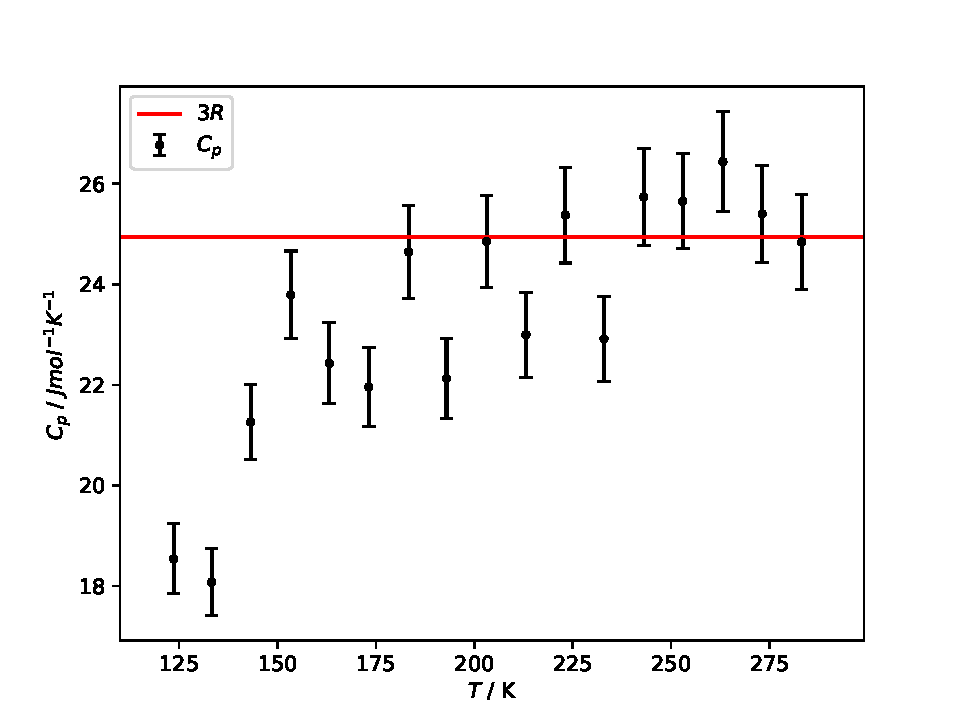
\includegraphics[scale=0.9]{fig/plot1.pdf}
	\caption{Die Molwärmen bei konstantem Druck in Abhängigkeit der Temperatur.}
	\label{fig:cp1}
\end{figure}
\FloatBarrier
\newpage
\noindent Als nächstes wird mithilfe von Gleichung (\ref{eqn:cv}) die Molwärme bei konstantem Druck $C_\mathrm{p}$ zu der Molwärme bei konstantem Volumen $C_\mathrm{V}$ umgerechnet.
Die Werte für $C_\mathrm{V}$ sind in Tabelle (\ref{tab:tab2}) angegeben.
\begin{table}
  \centering
  \caption{Daten für die Bestimmung der Molwärme bei konstantem Volumen $C_\mathrm{V}$.}
  \label{tab:tab2}
  \begin{tabular}{c c c c}
    \toprule
		$T$/K & $C_\mathrm{p}$ & $\alpha$ & $C_\mathrm{V}$ \\
    \midrule
    $123.63\pm0.24$ & $18.5\pm0.7$ & $\num{1.2500(22)e-05}$ & $18.4\pm0.7$ \\
    $133.27\pm0.24$ & $18.1\pm0.7$ & $\num{1.3391(22)e-05}$ & $17.9\pm0.7$ \\
    $143.18\pm0.24$ & $21.3\pm0.8$ & $\num{1.4309(22)e-05}$ & $21.0\pm0.7$ \\
    $153.39\pm0.24$ & $23.8\pm0.9$ & $\num{1.5253(23)e-05}$ & $23.5\pm0.9$ \\
    $163.15\pm0.24$ & $22.4\pm0.8$ & $\num{1.6156(23)e-05}$ & $22.1\pm0.8$ \\
    $173.21\pm0.25$ & $22.0\pm0.8$ & $\num{1.7086(23)e-05}$ & $21.5\pm0.8$ \\
    $183.30\pm0.25$ & $24.6\pm0.9$ & $\num{1.8020(23)e-05}$ & $24.1\pm0.9$ \\
    $192.95\pm0.25$ & $22.1\pm0.8$ & $\num{1.8912(23)e-05}$ & $21.5\pm0.8$ \\
    $203.14\pm0.25$ & $24.9\pm0.9$ & $\num{1.9854(23)e-05}$ & $24.1\pm0.9$ \\
    $213.12\pm0.25$ & $23.0\pm0.8$ & $\num{2.0778(23)e-05}$ & $22.2\pm0.8$ \\
    $223.14\pm0.25$ & $25.4\pm1.0$ & $\num{2.1705(23)e-05}$ & $24.5\pm1.0$ \\
    $232.95\pm0.25$ & $22.9\pm0.8$ & $\num{2.2612(23)e-05}$ & $21.9\pm0.8$ \\
    $243.06\pm0.25$ & $25.7\pm1.0$ & $\num{2.3517(23)e-05}$ & $24.6\pm1.0$ \\
    $252.96\pm0.25$ & $25.7\pm0.9$ & $\num{2.4463(24)e-05}$ & $24.3\pm0.9$ \\
    $263.15\pm0.26$ & $26.4\pm1.0$ & $\num{2.5406(24)e-05}$ & $24.9\pm1.0$ \\
    $273.13\pm0.26$ & $25.4\pm1.0$ & $\num{2.6329(24)e-05}$ & $23.7\pm1.0$ \\
    $283.15\pm0.26$ & $24.8\pm0.9$ & $\num{2.7256(24)e-05}$ & $23.0\pm0.9$ \\

    \bottomrule
  \end{tabular}
\end{table}
\FloatBarrier
\newpage
\noindent In Abbildung (\ref{fig:cv1}) sind die Daten graphisch dargestellt.
\begin{figure}[h]
	\centering
	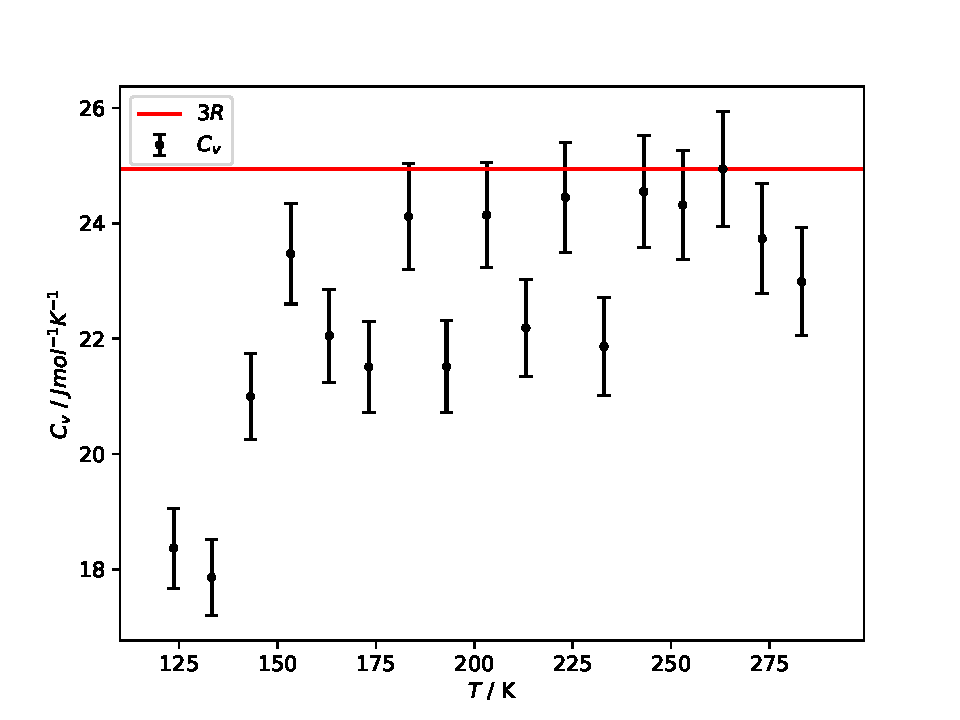
\includegraphics[scale=0.9]{fig/plot3.pdf}
	\caption{Die Molwärmen bei konstantem Volumen in Abhängigkeit der Temperatur.}
	\label{fig:cv1}
\end{figure}
\FloatBarrier
\noindent Die Einheiten für $C_\mathrm{V}$ und $C_\mathrm{p}$ sind gegeben durch:
\begin{equation*}
	[C_\mathrm{V}] = [C_\mathrm{p}] = \si{\joule\per\mole\per\kelvin}\,\text.
\end{equation*}

\subsection{Bestimmung der Debye-Temperatur}
Im letzten Auswertungsabschnitt soll nun noch die Debyetemperatur $\Theta_\mathrm{D}$ bestimmt werden, dabei wird ein experimenteller als auch ein theoretischer Wert erhalten.
\subsubsection{Experimentelle Bestimmung}
Zur experimentellen Bestimmung der Debye-Temperatur werden ausschließlich die Molwärmen $C_\mathrm{V}$ mit $T<\SI{170}{\kelvin}$ betrachtet.
Die Quotienten $\Theta_\mathrm{D} / T$ werden für ein gegebenes $C_\mathrm{V}$ aus der Debye-Funktion aus der Versuchsanleitung \cite[2,3]{Anleitung} ausgelesen.
Durch einfache Multiplikation kann dann die Debye-Temperatur bestimmt werden. In Tabelle \ref{tab:tab3} sind die daraus resultierenden Werte dargestellt.
\begin{table}
  \centering
  \caption{Daten zur Bestimmung der Debyetemperatur $\Theta_\mathrm{D}$.}
  \label{tab:tab3}
  \begin{tabular}{c c c c}
    \toprule
		$C_\mathrm{V}$ & $\Theta_\mathrm{D} / T$ & $T$/K & $\Theta_\mathrm{D}$/ \\
    \midrule
    $18.4\pm0.7$ & $2.6$ & $123.63\pm0.24$ & $321.4\pm0.6$ \\
    $17.9\pm0.7$ & $2.6$ & $133.27\pm0.24$ & $346.5\pm0.6$ \\
    $21.0\pm0.7$ & $1.9$ & $143.18\pm0.24$ & $272.0\pm0.5$ \\
    $23.5\pm0.9$ & $1.2$ & $153.39\pm0.24$ & $184.07\pm0.29$ \\
    $22.1\pm0.8$ & $1.6$ & $163.15\pm0.24$ & $261.0\pm0.4$ \\
    $21.5\pm0.8$ & $1.7$ & $173.21\pm0.25$ & $294.4\pm0.4$ \\
    \bottomrule
  \end{tabular}
\end{table}
\FloatBarrier
\noindent Daraus ergibt sich für die Debyetemperatur:
\begin{equation*}
  \overline{\Theta}_\mathrm{D}=\SI{279.9(2)}{\kelvin}
\end{equation*}
\subsubsection{Theoretische Bestimmung}
Aus Gleichung (\ref{eqn:Eigenschwingungen}) lässt sich die Debye-Frequenz berechnen.
Dafür werden zunächst die Größen $L^3$ und $N_L$ berechnet.
Die Geschwindigkeiten $v_\mathrm{long}$ und $v_\mathrm{trans}$ die dafür benötigt werden finden sich in der Versuchsanleitung \cite{Anleitung}. Diese sind gegeben durch:
\begin{align*}
  v_\mathrm{long} &= \SI{4700}{\meter\per\second} \\
  v_\mathrm{trans} &= \SI{2260}{\meter\per\second}
\end{align*}
Die Teilchenzahl lässt sich durch den Zusammenhang
\begin{equation}
  N_\mathrm{L} = \dfrac{m}{M} \cdot N_\mathrm{A}
\end{equation}
berechnen.
Das Volumen $L^3$ wird bestimmt aus:
\begin{equation}
  L^3 = V = V_0 \cdot \frac{m}{M}
\end{equation}
Daraus folgt die Debye-Frequenz mit $\omega_\mathrm{D} = \SI{43.54e12}{\hertz}$.
Mithilfe der folgenden Gleichung,
\begin{equation}
  \Theta_\mathrm{D} =\dfrac{\hbar\cdot\omega_\mathrm{D}}{k_\mathrm{B}}
\end{equation}
wird die Debye-Temperatur zu $\Theta_\mathrm{D} = \SI{332.57}{\kelvin}$ bestimmt.
